\section{Applying the Fourier transform on the image}\label{P4}

For the purpose of determining the appearance of the magnitude (log) of the modified image, the Fourier transform, the low-pass Gaussian filter, and the sharpening filter are all applied to the image in this section. Given the information presented in Figure 11, it is possible to make the observation that the Fourier transform of a low pass Gaussian filter results in a Gaussian filter that has a bigger standard deviation. 

\begin{figure}[h]
    \centering
    \begin{subfigure}{0.4\textwidth}
        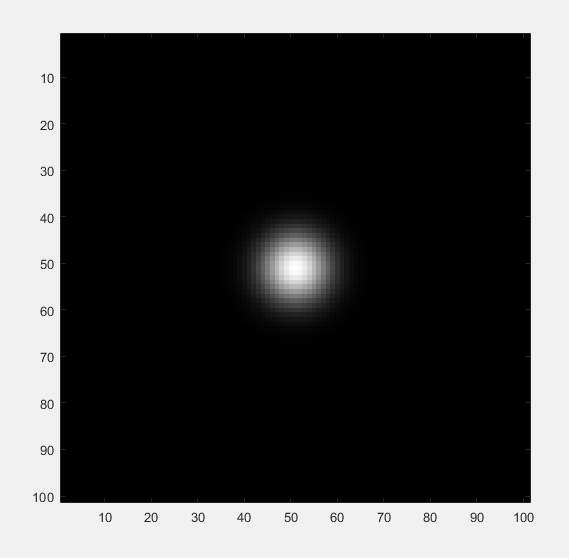
\includegraphics[width=\textwidth]{Resources/F11-a.png}
        \caption{}
        \label{fig:first}
    \end{subfigure}
    \hfill
    \begin{subfigure}{0.4\textwidth}
        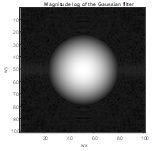
\includegraphics[width=\textwidth]{Resources/F11-b.png}
        \caption{}
        \label{fig:Second}
    \end{subfigure}
    \caption{Low-pass Gaussian filter image and magnitude log of the Fourier transform}
    \label{fig:Fourier transform}
\end{figure}